\section{Introduction}
%\paragraph{Motivation: ML + Fairness}
Machine learning (ML) is becoming the omnipresent technology of our time. 
ML algorithms are being used for high-stake decisions like college admissions, crime recidivism, insurance, and loan decisions.
Thus, human lives are now pervasively influenced by data, ML, and their inherent bias.

\begin{example}\label{fairness_justicia_example:intro}
Let us consider an example (Figure~\ref{fairness_justicia_fig:fair_example}) of deciding eligibility for health insurance depending on the fitness and income of the individuals of different age groups (20-40 and 40-60).
Typically, incomes of individuals increase as their ages increase while their fitness deteriorates.
We assume relation of income and fitness depends on the age as per the Normal distributions in Figure~\ref{fairness_justicia_fig:fair_example}.
Now, if we train a decision tree~\cite{narodytska2018learning} on these fitness and income indicators to decide the eligibility of an individual to get a health insurance, we observe that the `optimal' decision tree (ref. Figure~\ref{fairness_justicia_fig:fair_example}) selects a person above and below $40$ years with probabilities $0.18$ and $0.72$ respectively.
This simple example demonstrates that even if an ML algorithm does not explicitly learn to differentiate on the basis of a sensitive attribute, it discriminates different age groups due to the utilitarian sense of accuracy that it tries to optimize.
\end{example}

\begin{figure}[t!]
	\centering
	\begin{minipage}{.18\columnwidth}
		\centering
		\scalebox{0.5}{	
			\begin{tikzpicture}[x=1.5cm,y=1.8cm]
			% Define nodes
			\node[latent,scale=1.5] (a1) {$\textrm{age}$} ; %
			\node[obs, scale=1.5, below=of a1, xshift=-.6cm] (h) {$\textrm{fitness}$}; %
			\node[obs, scale=1.5, below=of a1, xshift=.6cm] (i) {$\textrm{income}$}; %
			\node[obs, scale=1.5, below=of h, xshift=.6cm] (p) {$\hat{Y}$}; %			
			%%add edge
			\edge[] {a1} {h,i} ;
			\edge[] {h,i} {p} ;
			\end{tikzpicture}
		}
	\end{minipage}\hfill
	\begin{minipage}{.2\columnwidth}
		\centering
		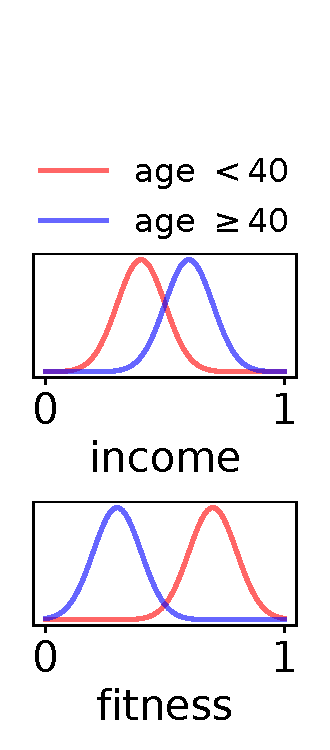
\includegraphics[scale=0.35]{figures/fairness/justicia/example.pdf}
	\end{minipage}\hfill
	\begin{minipage}{.5\columnwidth}
		\scalebox{0.37}{	
			\begin{tikzpicture}[x=1cm,y=1.8cm]
			\node [box, scale=2]                                    (p)      {fitness $\geq 0.61$};
			\node [scale=2, above= -0.1cm of p]  (a)    {Trained Decision Tree};
			\node [scale=2, box, below=  -1cm of p, xshift=-1.4cm]    (a1)    {income\\ $\geq 0.29$};
			\node [scale=2, box, below= -1cm of p, xshift=1.4cm]     (a2)    {income $\geq 0.69$};
			\node [scale=2,below= of a1, xshift=-1.2cm]  (a11)    { $1$};
			\node [scale=2,below= of a1, xshift=1.2cm]   (a12)    { $0 $};
			\node [scale=2,below= of a2, xshift=-1.2cm]  (a21)    { $1$};
			\node [scale=2,below= of a2, xshift=1.2cm]  (a22)    { $0$};
			%
			\path [line] (p) -|         (a1) node [scale=1.5,midway, above]  {Y};
			\path [line] (p) -|         (a2) node [scale=1.5,midway, above]  {N};
			\path [line] (a1) -|       (a11) node [scale=1.5,midway, above]  {Y};
			\path [line] (a1) -|       (a12) node [scale=1.5,midway, above]  {N};
			\path [line] (a2) -|       (a21) node [scale=1.5,midway, above]  {Y};
			\path [line] (a2) -|       (a22) node [scale=1.5,midway, above]  {N};
			\end{tikzpicture}}
	\end{minipage}%
	\caption{A trained decision tree to learn eligibility for health insurance using age-dependent fitness and income indicators.}\label{fairness_justicia_fig:fair_example}

\end{figure}
\subsubsection{Fair ML.} Statistical discriminations caused by ML algorithms have motivated researchers to develop several frameworks to ensure fairness and several algorithms to mitigate bias.
Existing fairness metrics mostly belong to three categories: \textit{independence}, \textit{separation}, and \textit{sufficiency}~\cite{mehrabi2019survey}. 
Independence metrics, such as demographic parity, statistical parity, and group parity, try and ensure the outcomes of an algorithm to be independent of the groups that the individuals belong to~\cite{feldman2015certifying,dwork2012fairness}.
Separation metrics, such as equalized odds, define an algorithm to be fair if the probability of getting the same outcomes for different groups are same~\cite{hardt2016equality}.
Sufficiency metrics, such as counterfactual fairness, constrain the probability of outcomes to be independent of individual's sensitive data given their identical non-sensitive data~\cite{kusner2017counterfactual}. %,wu2019counterfactual

In Figure~\ref{fairness_justicia_fig:fair_example}, independence is satisfied if the probability of getting insurance is same for both the age groups. Separation is satisfied if the number of `actually' (ground-truth) ineligible and eligible people getting the insurance are same. Sufficiency is satisfied if the eligibility is independent of their age given their attributes are the same.
Thus, we see that the metrics of fairness can be contradictory and complimentary depending on the application and the data~\cite{corbett2018measure}.
Different algorithms have also been devised to ensure one or multiple of the fairness definitions.
These algorithms try to rectify and mitigate the bias in the data and thus in the prediction-model in three ways: \textit{pre-processing} the data~\cite{kamiran2012data,zemel2013learning,calmon2017optimized}, \textit{in-processing} the algorithm~\cite{zhang2018mitigating}, and \textit{post-processing} the outcomes~\cite{kamiran2012decision,hardt2016equality}.

\subsubsection{Fairness Verifiers.} Due to the abundance of fairness metrics and difference in algorithms to achieve them, it has become necessary to verify different fairness metrics over datasets and algorithms. 

In order to verify fairness as a model property on a dataset, verifiers like \textit{FairSquare}~\cite{albarghouthi2017fairsquare} and \textit{VeriFair}~\cite{bastani2019probabilistic} have been proposed. 
%FairSquare verifies demographic parity and individual fairness as a numerical integration problem for a specific program semantics.
%VeriFair translates fairness metrics to an enumeration problem of a specified Boolean syntax.
%These papers operate for a specific Boolean sensitive attribute.
These verifiers are referred to as {\em distributional verifiers} owing to the fact that their inputs are a probability  distribution of the attributes in the dataset and a model of a suitable form, and their objective is to verify fairness w.r.t. the distribution and the model.
Though FairSquare and VeriFair are robust and have asymptotic convergence guarantees, we observe that they scale up poorly with the size of inputs and also do not generalize to non-Boolean and compound sensitive attributes.
In contrast to the distributional verifiers, another line of work, referred to as sample-based verifiers, has focused on the design of testing methodologies  on a given fixed data sample~\cite{galhotra2017fairness,aif360-oct-2018}. 
Since sample-based verifiers are dataset-specific, they generally do not provide robustness over the distribution.


%\blue{Other papers: Probabilistic Verification of Fairness Properties via	Concentration, Verifying Individual Fairness in Machine Learning Models~\cite{john2020verifying}}
Thus, a \textit{unified formal framework} to verify \textit{different fairness metrics} of an ML algorithm, which is \textit{scalable}, capable of \textit{handling compound protected groups}, \textit{robust} with respect to the test data, and \textit{operational on real-life} datasets and fairness-enhancing algorithms, is missing in the literature.

\subsubsection{Our Contribution.} From this vantage point, \textit{we propose to model verifying different fairness metrics as a Stochastic Boolean Satisfiability (SSAT) problem}~\cite{littman2001stochastic}.
SSAT was originally introduced by ~\cite{papadimitriou1985games} to model {\em games against nature}. In this work, we primarily focus on reductions to the exist-random quantified fragment of SSAT, which is also known as E-MAJSAT~\cite{littman2001stochastic}. 
SSAT is a conceptual framework that has been employed to capture several fundamental problems in AI such as computation of maximum a posteriori (MAP) hypothesis~\cite{fremont2017maximum},  propositional probabilistic planning~\cite{majercik2007appssat},  and circuit verification~\cite{lee2018towards}.
Furthermore, our choice of SSAT as a target formulation is motivated by the recent algorithmic progress that has yielded efficient SSAT tools~\cite{lee2017solving,lee2018solving}.



%We formulate SSAT encodings of the fairness verification problems and two methods to evaluate them in order to verify independence and separation metrics for any supervised learning algorithm using a unified scheme.
%Our encodings not only allow us to compute for non-Boolean and compound sensitive attributes but also to scale significantly better than existing formal verifiers. 
%We perform experimental analysis for multiple fairness metrics, datasets, and algorithms to instantiate the efficiency and effectiveness of our approach.

Our contributions are summarised below:
\begin{itemize}
	\item We propose a unified SSAT-based approach, {\justicia}, to verify independence and separation metrics of fairness for different datasets and classification algorithms.
	%\item \blue{{\justicia} measures fairness metrics for pre-, in-, and post-processing algorithms with respect to the data  generating distribution}.
	\item Unlike previously proposed formal distributional verifiers, namely FairSquare and VeriFair, {\justicia} verifies fairness for compound and non-Boolean sensitive attributes.%, and also \red{separation metrics}.
	\item Our experiments validate that our method is more accurate and scalable than the distributional verifiers, such as FairSquare and VeriFair, and more robust than the sample-based empirical verifiers, such as AIF360.
	\item We prove a finite-sample error bound on our estimated fairness metrics which is stronger than the existing asymptotic guarantees.
\end{itemize}

It is worth remarking that significant advances in AI bear testimony to the right choice of formulation, for example, formulation of planning as SAT~\cite{kautz1992planning}. In this context, we view that formulation of fairness as SSAT has potential to spur future work from both the modeling and encoding perspective as well as core algorithmic improvements in the underlying SSAT solvers.  

\iffalse
With this growing set of algorithms and definitions, it has become important to measure and verify fairness and bias of different algorithms and datasets. 
One popular approach is to use specific test dataset to compute the related statistical quantities and to certify fairness for that specific test dataset.
AIF360~\cite{aif360-oct-2018} provides a unified framework to implement multiple algorithms and to measure their fairness depending on such test datasets.
Though this method of verification works for a specified datasets, such verifiers do not explain how much a fairness measure depends on which sensitive attribute and is not robust to the selection of test dataset and its size.
\fi